\documentclass{article}

\usepackage[final]{nips_2016}
\usepackage[utf8]{inputenc} % allow utf-8 input
\usepackage[T1]{fontenc}    % use 8-bit T1 fonts
\usepackage{hyperref}       % hyperlinks
\usepackage{url}            % simple URL typesetting
\usepackage{booktabs}       % professional-quality tables
\usepackage{amsfonts}       % blackboard math symbols
\usepackage{nicefrac}       % compact symbols for 1/2, etc.
\usepackage{microtype}      % microtypography
\usepackage{enumerate}	% Use enumerate to list subsections
\usepackage{graphicx}	% Use pdf, png, jpg, or eps � with pdflatex; use eps in DVI mode
\usepackage{fancyvrb}
\usepackage{amsmath}
\usepackage{amsfonts}
\usepackage{dsfont}
\usepackage {tikz}
\usepackage{pgfplots}
\usepackage{pdflscape}
\usetikzlibrary {positioning}
\usepackage{float}
\setlength{\belowcaptionskip}{-20pt}

\title{Exploiting Sparse and Low-rank Structure for Visual Saliency}
\author{
Quan Zhou \\
Department of Computer Science \\
Boston University \\
\texttt{kenzhou@bu.edu} \\
\And
Calvin Liang \\
Department of Computer Science \\
Boston University \\
\texttt{cyung20@bu.edu}  \\
\And
Michael Mangione \\
Department of Computer Science \\
Boston University \\
\texttt{mjdm@bu.edu}  \\
\And
Ravi K. Rajendran \\
Department of Computer Science \\
Boston University \\
\texttt{raviraj4@bu.edu}  \\
}
\begin{document}
\maketitle

\begin{abstract}
For our project, we are interested in exploring the functionality and effectiveness of two different salient object detection models when tested on videos in order to demonstrate how well these models - influenced by different compressive sensing methods - perform. We accomplished this objective by applying each model to every individual frame of a video, then merging the resulting saliency maps back into two videos to see how well the models detect and maintain the salient object(s). The first of our implementation is from the Hou's saliency model, which implements an algorithm based only on a spectral residual approach to generate a saliency map from RGB images. The second is known as the Low-rank and Structured sparse Matrix Decomposition (SMD) model which uses low-rank and structured-sparsity regularization for image backgrounds and salient objects, respectively. This model first extracts features from an image (such as textures and colors) into a matrix, and takes prior knowledge (such as location and background) to form a high-level prior map. It then decomposes the feature matrix F into the summation of a low-rank part $\bf{L}$ and a structured-sparse $\bf{S}$ separating the salient object from the background and producing the saliency map. After computing each model's saliency maps, we conclude that the SMD model is superior.
\end{abstract}

\section{Introduction}
Over the years, visual saliency has emerged as a topic of great interest for researchers in multiple domains, such as the neuroscience and computer vision fields. There are a multitude of applications derived from visual saliency that are used to discuss and solve problems, such as signal processing, pattern recognition, and salient object detection. For our project, we focused specifically on the application of the latter and applied two differing models on a series of videos in order to observe the expected discrepancies in the accuracies of their results. \\
Salient object detection involves taking an image, or a series of images, and being able to detect and extract objects based on how much they stand out with respect to their background and surroundings. Such features include differing colors and orientations. The resulting output is the detected object, which is also referred to as the saliency map. There are many models in compressive sensing that are used to compute these saliency maps, but the two most common information processing approaches are known as the bottom-up and top-down models. The former is a stimulus-driven process in which an object is identified using features that distinguish the object from its surroundings (ie. color, texture, and location). In contrast, the latter is a task-driven process that utilizes prior knowledge of an image (ie. context and background) as a guide for computation. A common practice for computing saliency is implementing an amalgamation of both models by using low-level features and high-level prior knowledge in order to produce a low-rank matrix recovery (LR) model. Existing LR models typically agree that images are composed of two major features: (1) the background which is represented as highly redundant information, and (2) a sparse salient foreground object.\\
However, while the LR-model is frequently used as a basis for computing saliency maps, it is clearly far from perfect because it ultimately neglects the underlying structure of images, and inevitably degrade[s] the associated performance. Spatial relations, such as spatial contiguity and pattern consistency, between foreground pixels and patches are ignored, so it's incredibly difficult to separate or distinguish objects from backgrounds that contain similar features (eg. color). This results in a typically blurry saliency map that can capture objects' general geometric outlines, but fail to produce the definition necessary to identify what these objects are. This is especially difficult for foreground objects that are perceptually similar to their backgrounds. Therefore as a solution to this limitation, we will implement a low-rank and structured matrix decomposition model (SMD), as proposed by Ling et al [1], that will utilize both low-rank and structured-sparse matrices to better separate objects in the foreground from the image's background. The low-rank matrix recovery problem is as follows: \\
\begin{center}
$\min_{L,S}\psi (L) + \alpha \omega (S) + \beta \theta (L ,S)$ s.t. F = L + S
\end{center}
where $\psi(\cdot)$ is a low-rank constraint to allow identification of the intrinsic feature subspace of the redundant background patches, $\omega(\cdot)$ is a structured sparsity regularization to capture the spatial and feature relations of patches in S, $\theta(\cdot, \cdot)$ is an interactive regularization term to enlarge the distance between the subspaces drawn from L and S, and $\alpha$, $\beta$ are positive tradeoff parameters. With this, we can take the feature matrix F of an input image and decompose it into a low-rank matrix part L (which represents the redundant information and non-salient background) plus a sparse matrix part S (which represents the salient objects in the foreground).\\
Hou's model [2], unlike SMD, is independent of features and prior knowledge of objects when it computes a saliency map. Instead, the model focuses on simulating pre-attentive processing observed in the human visual system. That is, it detects low level features such as orientation of the object or edges before identifying what the object is. The resulting detected object is what Hou and Zhang refer to as a proto-object. Hou's model is primarily a matrix decomposition given a precomputed average log spectrum curve for natural images. Such a matrix decomposition can be seen as a normalization of the frequency domain. The log spectrum of the input image is analyzed in order to obtain the spectral residual, which is then transformed to spatial domain in order to create a saliency map of the proto-object's general position.\\
Hou's model works well for salient objects that are comprised of a single frequency. In fact, it has the capacity to correctly capture multiple salient objects, so long as the frequencies of the objects are significantly different from the majority of the image. This is akin to the incoherence condition for compressed sensing, and as such a natural candidate for comparison with a refined compressed sensing model.\\

\section{Structured Matrix Decomposition (SMD)}
In order to improve upon the results of LR-models, we implement it along with the structured matrix decomposition model. The SMD is comprised of three parts: (1) Low-rank regularization for image background; (2) Structured-sparsity regularization for salient objects; and (3) Laplacian Regularization. 
Provided that background image patches often share similar features and lie in a low-dimensional subspace, low-rank regularization onto the feature matrix L is appropriate in order to eliminate any redundant information so we may obtain L's intrinsic low-dimensional structure. This is done by taking the nuclear norm of L as a convex relaxation, as illustrated in the following equation:\\
\[\psi (L) = rank(L) = \|L\|_{*} + \epsilon\]
where $\epsilon$ represents the relaxation error. \\
Next, we implement a tree-structured sparsity-inducing norm to encode the spatial relations between image patches that were ignored in LR-models. The tree-structured sparsity regularization is represented by the following equation:
\begin{align*}
\Omega \left( S \right) = \sum_{i=1}^d \sum_{j=1}^{n_i} v_j^i \Vert S_{G_j^i} \Vert_p
\end{align*}
\newline
where  $v_{j}^i \geq 0$ is the weight for the node $G_{j}^i, S_{G_{j}^i} \in R^{D \times |G_{j}^i|}$ ($|\cdot|$ denotes set cardinality) is the sub-matrix of S corresponding to the node $G_{j}^i$, and $\|\cdot \|_p$ is the p-norm, $1 \leq p \leq \infty$. $\Omega(\cdot)$ is the weighted group sparsity norm defined over a tree structure that groups identical patches together and represents relationships between these groups. We use the l-infinity norm on $S_{G_{j}^i}$ in order to ensure that same-group patches within $S_{G_{j}^i}$ have identical saliency values. The maximum saliency value of these groups are then evaluated in order to determine whether the group is salient or not. \\
Lastly, we integrate Laplacian regularization on the low-rank and structured-sparse matrices in order to enlarge the distance between the feature subspaces induced by them. Given the assumption that two adjacent patches with similar features have close representations in the subspace, the following regularization is defined:\\
\[\theta (L,S) = \frac{1}{2} \sum_{i,j = 1}^{N} \|s_i - s_j\|_2^2w_{i,j} = \text{Tr}(SM_FS^T),\]
where $s_i$ denotes the i-th column of $S$, $w_{i,j}$ is the (i, j)-th entry of an affinity matrix $W = (w_{i,j}) \in R^{N\text{x}N} $ and represents the feature similarity of patches $(P_i, P_j)$, $Tr(\cdot)$ denotes the trace of a matrix, and $M_{F} \in R^{N\text{x}N}$ is a Laplacian matrix. The Laplacian Regularization, in effect, enables us to separate the salient object from the background with greater ease because the groups of patches are more differentiable given they have their own distinct homogeneous regions and representations. \\

\subsection{Optimization of SMD}
In order to solve the convex problem in our initial equation, we implement the alternating direction method (ADM). We start by making the objective function separable:

\begin{align*}
{min_{L,S}} = \Vert  L \Vert_{*} + \text{ } \alpha \sum_{i=1}^d \sum_{j=1}^{n_i} v_j^i | \Vert S_{G_j^i} \Vert_p + \beta Tr \left( HM_FH^T \right) \\ \textit{ s.t.  } F = L + S,  S = H
\end{align*}
\newline
After which, we minimize the following Lagrangian function:

\begin{align*}
\mathcal{L} (L, S, H, Y_1, Y_2, \mu) &= \Vert L \Vert_{*}  \\&+ \alpha \sum_{i=1}^d \sum_{j=1}^{n_i} v_j^i | \Vert S_{G_j^i} \Vert_p + \beta Tr(HM_FH^T)  \\&+ Tr(Y_1^T ( F- L- S)) + Tr(Y_2^T(S-H))  \\&+  \frac{\mu}{2} ( \Vert F-L-S \Vert_F^2 + \Vert S -H \Vert_F^2 )
\end{align*}

where $Y_1$ and $Y_2$ are the Lagrange multipliers, and $\mu > 0$ controls the penalty for violating the linear constraints. We iteratively perform minimizations onto L, H, and S, alternately updating each individual component with the other two components at fixed values until our algorithm converges and it returns the optimal L and S.

\section{SMD Overview}
The SMD process can be summed up in a series of four steps [1]: (1) Image Abstraction; (2) Tree Construction; (3) Matrix Decomposition; and (4) Saliency Assignment. \\
Step 1: We start by taking an input image and extracting its low-level features (such as color) and group them accordingly based on their homogeneous elements, which we subsequently use to create a 53-dimension feature space D. We then perform the simple linear iterative clustering (SLIC) algorithm in said feature space to over-segment the image into a series of N patches such that P = $\{P_1, P_2, \cdots, P_N\}$. Each patch is represented as a feature vector $f_i$, and when they're combined together, they form the feature matrix, which is represented as $F = [f_1, f_2, \cdots, f_N]$.\\
Step 2: We utilize the hierarchical segmentation method to construct an index tree that illustrates the structure of the input image. Patches that share similar or identical characteristics with their neighbors are merged together and a sequence of granularity-increasing segmentations is produced as a result. \\
Step 3: We perform the SMD model on our feature matrix F (obtained in the first part) and decompose it into a low-rank part L and a structured-sparse part S, thus separating any foreground objects with homogeneous patches from the non-salient background.\\
Step 4: We transfer our results from step three to the spatial domain so we may estimate the saliency value of each patch by performing the following function on the structured matrix S:\\
\[Sal(P_i) = \|s_i\|_1\]
where $s_i$ represents the i-th column of S. The values of each patch correspond to their likelihoods of belonging to the salient object, so the higher the value, the greater the chances of the patch being in the salient object. We then merge all the patches together to produce a saliency map with regions of differing saliency values - the one with the highest values being our salient object.\\

\begin{figure}[ht]
\centering
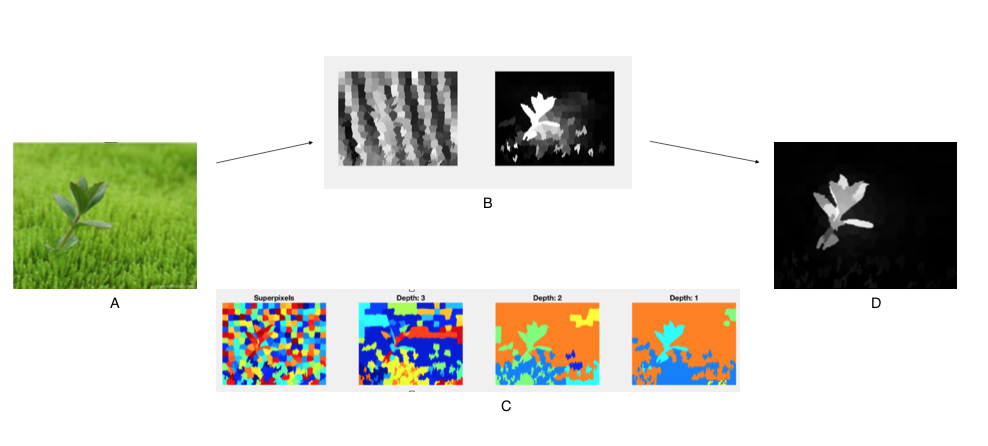
\includegraphics[scale = 0.8]{map.png}
\caption{SMD Overview}\hfill
\end{figure}

In Figure 1, A is the original input image to the SMD model. B represents the feature creation via top-down (left) and bottom up (right) feature evaluation. C is the super pixel generation, along with three depth iterations of super pixel linking as defined in the index tree creation protocol. D is the final output saliency, or the convolution of these two distinct feature mapping procedures.

\section{Video Saliency}
Video saliency is a natural and essential application of compressive sensing and image saliency computations, especially as live-video input becomes more commonplace in consumer electronics. Some solutions for this have already been devised, like the joint spatial saliency and optical flow temporal saliency map proposed by Ren et al.[3] Their algorithm combines the motion vectorization of objects between frames with traditional saliency computation techniques to produce an enhanced saliency mapping. Their developments point to an ever increasing need to optimize saliency creation routines for both accuracy and speed.

\section{Results}
\subsection{Evaluation Measures}
Following the same evaluation schemes adopted in Ling et al[1], we used Precision Recall(PR), Receiving Operating Characteristic(ROC) and weighted harmonic mean measure (F-measure) to compare the performance of the two models in this study.\\
\begin{enumerate}[1.]
\item \textsc{pr curve}\\
The formula definition for PR relations are shown below:\\
\[\text{Precision}=\frac{\text{True Positives}}{\text{True Positives} + \text{False Positives}}\]
\[\text{Recall}=\frac{\text{True Positives}}{\text{True Positives} + \text{False Negatives}}\]
Precision and Recall of the predictions are inversely related. When we examine the PR curve for any algorithm/model, we'd like to observe higher precision with lower recall.  
\\
\item \textsc{roc curve}\\
ROC curves compares the true positives rates (sensitivity of saliency) against false positives rates (1 - specificity). A model with curves as far away from the line $y=x$ is more desirable, indicating high sensitivity and high specificity and therefore better in saliency detection.
\\
\item \textsc{f-measure}\\
F-measure, or the arithmetic mean of precision and recall, is defined in the following equation:\\
\[F_{\beta} = \frac{(1+\beta^2)\times \text{Precision }+ \text{Recall}}{\beta^2 \times \text{Precision} + \text{Recall}}\]
F-measure tells how many instances are predicted correctly and the percentage of misses. A model may not perform well if its percentage of misses are high, even though its precision is high recall is low.

\end{enumerate}

\subsection{Comparison of Saliency Frames}
In Figure 3, a single static image and the corresponding Hou and SMD saliencies are presented.

\begin{figure}[H]
\centering
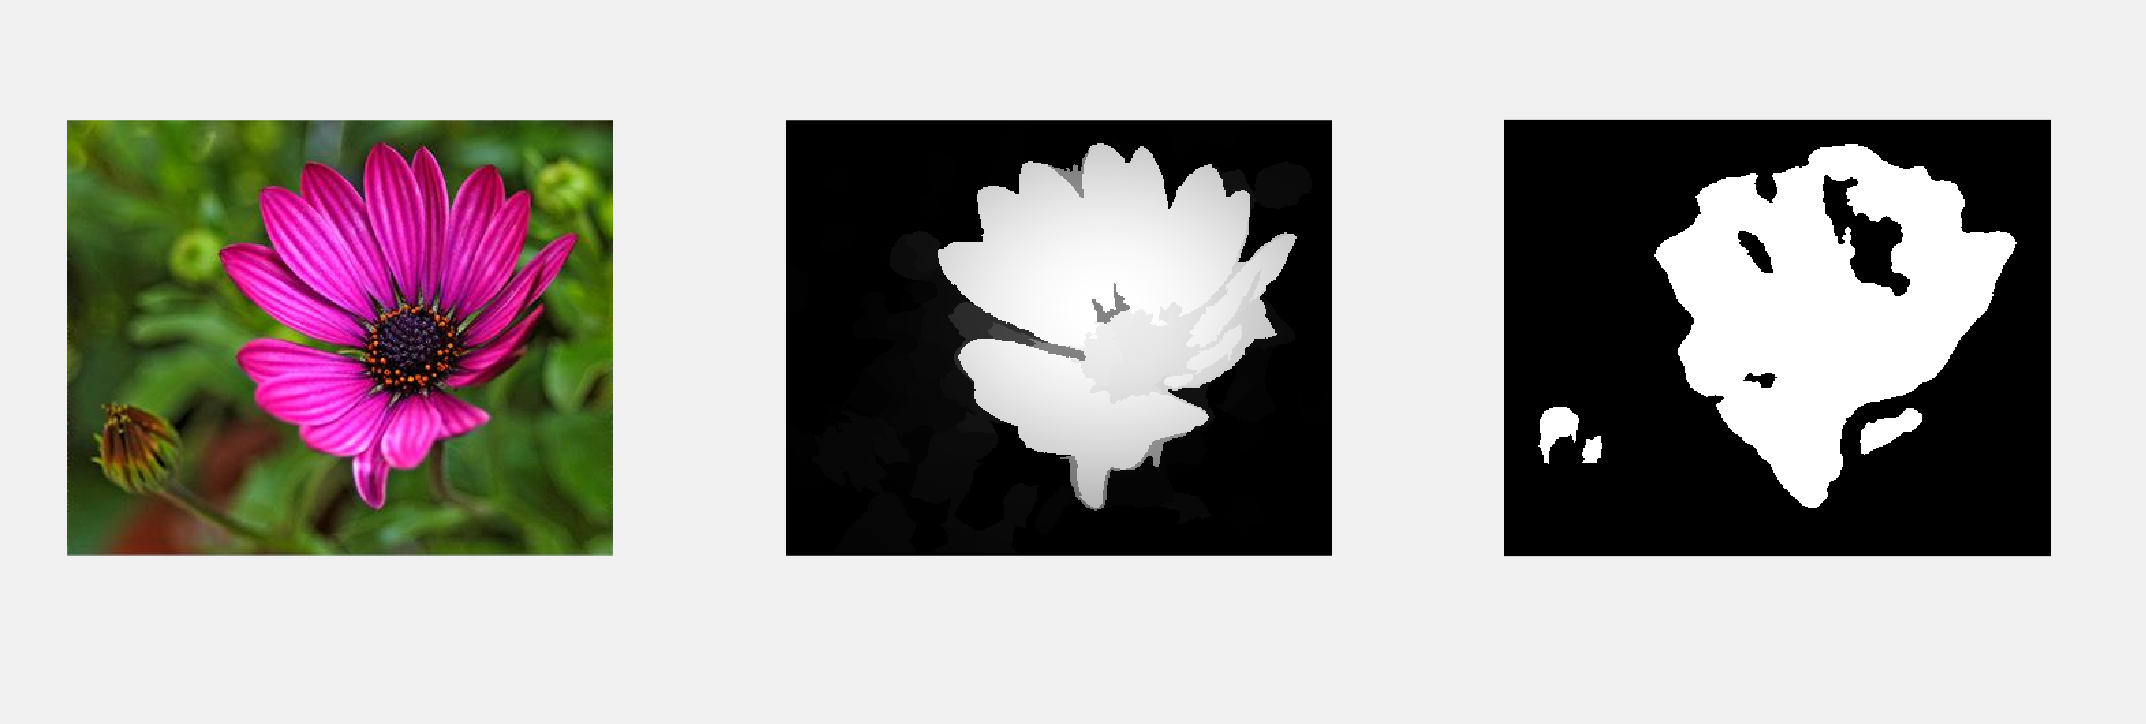
\includegraphics[scale = 0.35]{img-2.png}
\caption{Original image, Hou saliency, SMD saliency}\hfill
\end{figure}

Notice that the outline of the flower is captured in Hou, but important structural elements like the center and individual petals cannot be discerned. Since Hou works with frequencies and not structured super pixels, the resulting map has a distinct roundness on the edges, with makes for subpar mapping of the object. Hou also captures a completely distinct, yet not worthwhile, flower apart from the focal point of the image. In some domains, this could be considered a feature, since the second flower is relatively distinct from the background. However, the second flower has not structure, and fundamentally it is not considered in the ground truth.\\
SMD, on the other-hand, captures both the structure of the flower, its ground truth, and additional sub-structures in the flower. Even the ground truth does cannot discern the inner flower from the outer petals, which might be important for a sparse reconstruction of the image, depending on sampling limitations. Structure and detail are both included and well defined in SMD, whereas Hou makes sacrifices in detail for an output that does a poor job of capturing either. \\
It is worth noting that in this sample, Hou actually outperforms many of its other saliency predictions. The stark contrast in the color of the flower and the background, along with the relatively constant coloring of the non-salient area, gives Hou an advantage that it usually lacks. Indeed, these are similar to the sparse and incoherent requirements of compressed sensing, which would explain why Hou manages to perform reasonably. 

In Figure 3, we see the results of Hou and SMD saliency models for a sequence of frames depicting the demolition of  a tower. 

\begin{figure}[ht]
\centering
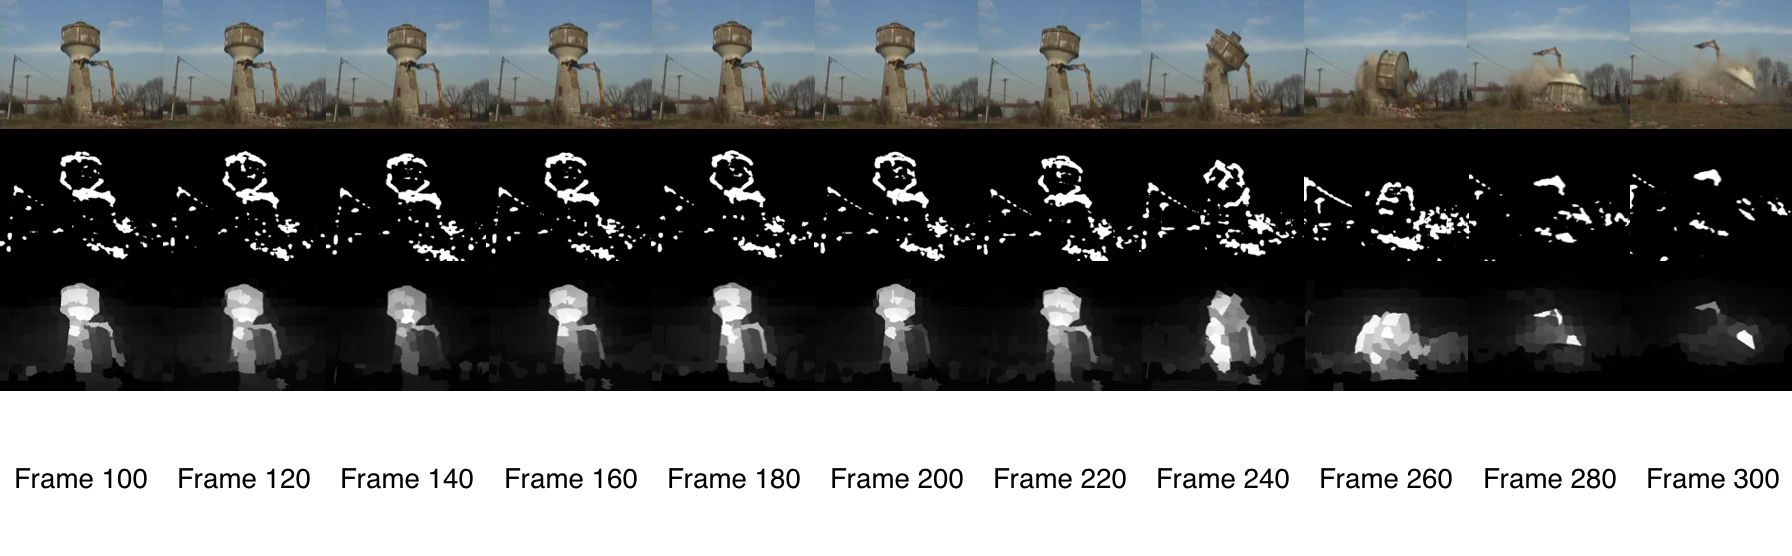
\includegraphics[scale = 0.4]{SaliencyFrames.png}
\caption{Comparison of the saliency by frames (30 frames per second)}\hfill
\end{figure}

Qualitatively, the difference between Hou and SMD is obvious. SMD produces a well structured, concise representation of the salient object (or objects, including the crane). The stray phone line captured by Hou is absent in SMD, and the base of the tower is captured sufficiently. Hou does not manage to fully identify a single object, instead capturing trace portions of features of the tower without fully representing the tower itself. SMD, however, fully captures the base and top of the tower, and additionally weights the elements of the structure by its striking features. Even the residual dust after the tower falls is proportionately captured in SMD, which should be considered salient on its own. Furthermore, the weighted super pixels in SMD provide a better groundwork for reconstruction, whereas the proto-objects in Hou lend no additional information about the importance of the regions captured.

\begin{figure}[ht]
\centering
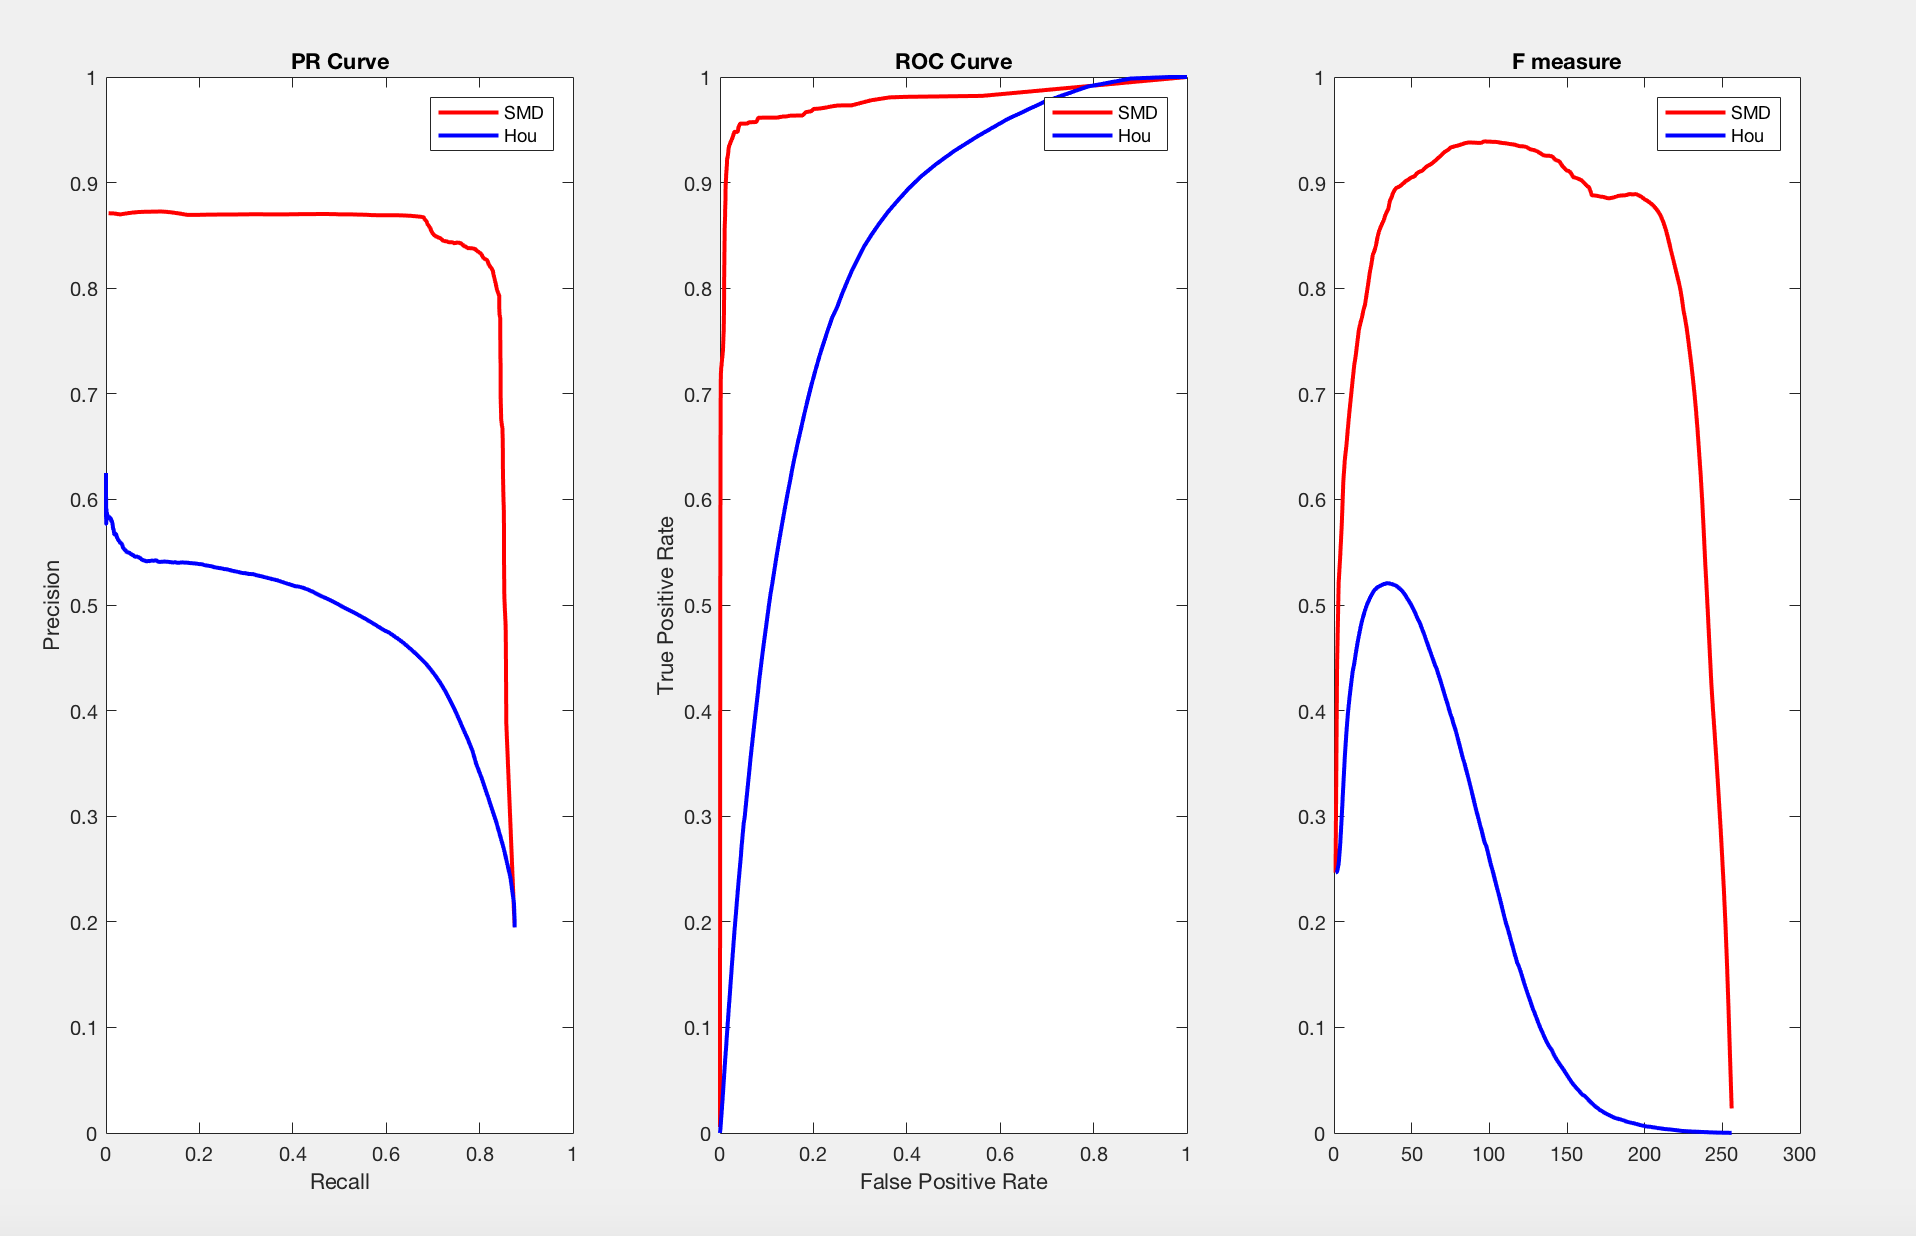
\includegraphics[scale = 0.4]{Evaluationcomparison.png}
\caption{Comparison of PR, ROC, and F-measure between Hou's Saliency and SMD Saliency }\hfill
\end{figure}

In Figure 3, we are presented the Precision Recall, Receiver Operating Characteristics, and F Measure curves for the two models, run against a series of 8 testing images (included in the Data repository).

Strictly regarding runtime, Hou performs exceptionally. For the set of images, the Hou saliency is able to compute all proto-object maps in a runtime $\leq$ 0.11 seconds on a 2015 Macbook Pro with an 2.7 GHz Intel Core i5 processor. This kind of real time computation makes the Hou model viable for problem domains where the rate of processing input is key. However, saliency evaluation amounts to much more than runtime alone, especially for object tracking. Even in static images, the accuracy of Hou is highly variable, and the objects it does manage to capture render the salient portion with low fidelity.

The runtime of SMD is significantly longer, but it is clear that this additional time is worthwhile. For the Precision recall curves, SMD produces a staggering level of precision up until a steep drop at 0.8 recall. At almost 0.9, SMD has a 0.3 precision lead on Hou at the least, with Hou trending down at an aggressive rate. SMD boasts a 0.95 ROC measure with no false positives, and almost attains a perfect 1 well before a false positive rate of 1. Hou makes logarithmic process on ROC, taking considerable accuracy loss to converge on a true positive rate of 1. The benefit of the SMD model is most clearly illustrated by the F measure curve, where Hou barely registers on the graph, let alone producing comparable results to SMD's near perfect precision and recall.

We can better understand the meaning of these curves in the context of the flower saliencies included in Figure 2. Across all three metrics, SMD performs extremely well. The Precision Recall for the flower is high with SMD, since the details of the flower are captured with a high degree of fidelity. The ROC is additionally high, because extraneous false features are not recorded (consider the un-blossomed flower to the bottom left one such false positive). The F measure is also high for SMD, as it produces high precision and lack of false positives together.

Hou manages to fail across these parameters with a high degree of consistency. Due to its use of averages, the precision recall is low and the flower lacks clarity around the edges. The Hou saliency has many false positives, as well as portions of the the salient flower that are missing that go missing in the output. The F measure reflects this general inaccuracy as one concise figure.
 
The Hou saliency outputs are a pertinent reminder of the a priori data features necessary to utilize compressed sensing. For Hou, the guarantee of sparsity and incoherence is needed in the frequency domain of the image. For example, an image of a halved grapefruit could be considered sparse, as it is a contained, circular half of the fruit,  and incoherent since the pink fruit is in opposition to the rest of the image composition. Hou captures this object well, because it sufficiently meets the compressed sensing criteria. However, in stark contrast, for the sample car destruction video, the input is neither sparse (no one frequency is dominant) nor incoherent (frequent color repetition across all parts of the frame). Hou captures some elements of the car, but with subpar accuracy. 

\section{Conclusion}
Ultimately SMD far surpasses the Hou model, and could conceivably be used for a number of salient model creation scenarios. It performs especially well with regard to contextual object structuring and low noise outputs. However, video processing presents many potential additions that can boost performance. For example, the vectorization of movement in the salient object between frames could result in a transferral of low-rank and structured sparse information for a given node in sequential super pixel trees. While not implemented, this extension is entirely feasible. That said, given a system with significant computational power, SMD will produce high-fidelity, feature rich saliencies that will make reconstruction straightforward. While baseline models like Hou and others are a good entry point, structured sparse matrix decompositions simply provide better results and incentivize the continued exploration of compressed sensing.

\section*{References}
\medskip

\small

[1] Peng H, \ \& Li B, \ \& Ling H, \ \& Hu W, \ \& Xiong W, \ \& Maybank SJ. \ (2014). Salient Object Detection via Structured Matrix Decomposition. Journal of Latex Class Files, VOL. 13, NO. 9

[2] Hou X, \ \& Zhang L. \ (2007). Saliency Detection: A Spectral Residual Approach. In: Proceedings CVPR '07, vol. 1, pp. 1-8

[3] Zhong S, \ \& Liu Y, \ \& Ren F, \ \& Zhang J, \ \& Ren R. (2013)  Video Saliency Detection via Dynamic Consistent Spatio-temporal Attention Modelling. In AAAI.

[4] Achanta R, \ \& Hemami S \ \& Estrada F \ \& Su?sstrunk S. \ (2009). Frequency-tuned salient region detection. In Proc. of CVPR, 1597?1604.				 

\end{document}

